%% LyX 2.3.7 created this file.  For more info, see http://www.lyx.org/.
%% Do not edit unless you really know what you are doing.
\documentclass[10pt,twocolumn,english,format=sigplan,screen,balance]{acmart}
\usepackage{fontspec}
\setmonofont{APL385 Unicode}
\setcounter{secnumdepth}{3}
\setcounter{tocdepth}{3}
\usepackage{array}
\usepackage{prettyref}
\usepackage{booktabs}
\usepackage{multirow}
\usepackage{graphicx}
\usepackage{rotating}
\ifx\hypersetup\undefined
  \AtBeginDocument{%
    \hypersetup{unicode=true}
  }
\else
  \hypersetup{unicode=true}
\fi

\makeatletter

%%%%%%%%%%%%%%%%%%%%%%%%%%%%%% LyX specific LaTeX commands.


\setcopyright{rightsretained}


\acmDOI{10.1145/3589246.3595371}


\acmYear{2023}


\copyrightyear{2023}


\acmSubmissionID{pldiws23arraymain-p5-p}


\acmISBN{979-8-4007-0169-6/23/06}


\acmConference[ARRAY '23]{Proceedings of the 9th ACM SIGPLAN International Workshop on Libraries, Languages and Compilers for Array Programming}{June 18, 2023}{Orlando, FL, USA}



\received{2023-03-31}


\received[accepted]{2023-04-21}

\newcommand{\noun}[1]{\textsc{#1}}
%% Because html converters don't know tabularnewline
\providecommand{\tabularnewline}{\\}

%%%%%%%%%%%%%%%%%%%%%%%%%%%%%% User specified LaTeX commands.

\usepackage{dblfloatfix}

\makeatother

\usepackage{polyglossia}
\setdefaultlanguage[variant=american]{english}
\begin{document}
\acmBooktitle{Proceedings of the 9th ACM SIGPLAN International Workshop on Libraries, Languages and Compilers for Array Programming (ARRAY '23), June 18, 2023, Orlando, FL, USA}

\acmPrice{}
\begin{CCSXML}
<ccs2012>
  <concept>
    <concept_id>10011007.10011006.10011008.10011009.10010175</concept_id>
    <concept_desc>Software and its engineering~Parallel programming languages</concept_desc> 
    <concept_significance>500</concept_significance>
  </concept>
  <concept>
    <concept_id>10011007.10011006.10011041.10011048</concept_id>
    <concept_desc>Software and its engineering~Runtime environments</concept_desc>
    <concept_significance>500</concept_significance>
  </concept>
</ccs2012>
\end{CCSXML}
\ccsdesc{Software and its engineering~Parallel programming languages}

\ccsdesc{Software and its engineering~Runtime environments}

\keywords{APL, Compilers, Neural Networks, Machine Learning, GPU, Co-dfns}
\title{U-Net CNN in APL}
\subtitle{Exploring Zero-Framework, Zero-Library Machine Learning}
\author{Aaron W. Hsu}
\email{aaron@dyalog.com}
\orcid{0000-0001-9292-7783}
\affiliation{\institution{Dyalog, Ltd.}\city{Bloomington, IN}\country{United States}}
\author{Rodrigo Girão Serrão}
\email{rodrigo@dyalog.com}
\orcid{0009-0009-3361-3835}
\affiliation{\institution{Dyalog, Ltd.}\city{Bramley}\country{United Kingdom}}
\begin{abstract}
The APL notation would appear to be a clear match for convolutional
neural networks, but traditional implementations of APL have lagged
behind the performance of highly tuned, specialized frameworks designed
to execute CNNs on the GPU. Moreover, most demonstrations of APL for
neural networking have involved relatively small examples. We explore
a more complex example in the U-net architecture and utilize a modern
APL compiler with GPU support, Co-dfns, to compare the state of the
art of APL against the current crop of specialized neural network
frameworks in the form of PyTorch. We compare performance as well
as the language design of APL for neural network programming and the
clarity and transparency of the resulting code. 

We found that the complete “from scratch” APL source was on
par with the complexity of the PyTorch reference implementation, albeit
more foreign, while being more concise and complete. We also found
that when compiled with Co-dfns, despite the naïve implementation
both of Co-dfns and our own code, performance on the GPU and the CPU
were within a factor of 2.2 - 2.4 times that of the PyTorch implementation.
We believe this suggests significant avenues of future exploration
for machine learning language design, pedagogy, and implementation,
both inside and outside of the APL community. 
\end{abstract}
\maketitle

\section{Introduction}

Specialized machine learning frameworks dominate present deep learning
applications. A wide number of highly specialized, optimized libraries
exist. These systems are more complex than typical libraries and are
better thought of as domain-specific languages (DSLs). While these
libraries bolster the current machine learning explosion, because
of their highly specialized nature, users tend to become specialists
around a very specific framework for computation. This creates a sharp
wall that impedes skills transference, where experts can use frameworks
effectively but may be under-prepared to handle situations that benefit
from broader or more flexible skill-sets.\footnote{To someone who only has a hammer, everything looks like a nail.}
This specialization makes sense in the context of traditional programming,
where simple networks are accessible, but tedious, while non-trivial
ML architectures quickly strain the performance and usability of a
“from scratch” implementation. This creates a sharp contrast
between simple systems programmed “by hand” and opaque, complex
frameworks that work as inflexible black boxes. A lack of profound
and intuitive understanding of the underlying mechanics of deep learning
systems fosters a type of “programming by knob turning” where
networks are programmed via trial and error rather than intentionality,
further exacerbating the danger of unintended consequences, already
an inherent difficulty in statistical ML \citep{domingos2012few}.
Machine learning frameworks are often highly vendor-specific; even
vendor-neutral systems encode greater specificity than warranted for
long-running code. This demands higher levels of programmer investment
in system maintenance over a product lifetime. Despite this, specialist
frameworks prove highly effective, in part because of the performance
demands of ML. However, in recent years, reemerging general-purpose
array programming languages have presented an alternative potential
direction. Such languages were popular during early neural network
programming in the 20th century \citep{alfonseca-1990-aplnn}, but
performance of then-current hardware prevented further development.

APL, a general-purpose array programming language, created by Kenneth
Iverson as an improved mathematical notation \citep{apl}, has risen
in popularity over the past decades, in part because of the renewed
interest in parallel computation and a wider acceptance of the use
of a variety of programming languages. Recently, new research into
APL as a machine learning language has begun. APL's origins in education
and its reputation for direct algorithmic expression \citep{knuth1993computer,knuth2007computer}
address some of the above concerns around general-purpose languages
and ML. As a linguistically stable language that is both high performance
and high level \citep{hsu2019data}, it is suitable for long lived
code as well as rapid prototyping, and the data-parallel by default
semantics suggests obvious applications to GPU programming. While
these advantages might recommend APL for machine learning, the majority
of implementations have run on the CPU only, usually via interpreter.
While challenging to compile, recent innovations to the language (particularly
those with a functional programming focus) make compilation more tractable,
and the Co-dfns compiler now exists as an APL implementation with
native GPU support \citep{hsu2019data}. 

Given the available APL technology and the paucity of existing research
on modern ML in APL, we explored APL as a ML language in terms of
language design and runtime performance by implementing and benchmarking
the U-net convolutional neural network \citep{unet}. This is a popular
image segmentation architecture with a particularly interesting U-shaped
design. It makes use of a range of popular CNN vocabularies and functions
while having a clear, non-trivial architecture. This makes an ideal
candidate for exploring APL's capabilities.

We make the following contributions:
\begin{itemize}
\item A from scratch implementation of the U-net convolutional neural network
in APL
\item Our U-net implementation is exceptionally simple, concise, transparent,
and direct
\item Our implementation consists of pure APL and no dependencies, frameworks,
libraries, or other supporting code
\item Performance results of two modern APL implementations, one compiled
and the other interpreted, on CPU and GPU hardware against a reference
PyTorch implementation for U-net
\end{itemize}

\section{Background}

\subsection{Convolutional Neural Networks}

The experiment this paper uses to produce its benchmarks is the reproduction
of a well-known convolutional neural network architecture. The use
of CNNs in machine learning was widely popularized with the publication
of a paper \citep{cnns-imagenet} that used CNNs to achieve state-of-the-art
performance in labeling pictures of the ImageNet \citep{imagenet}
challenge. However, a prominent paper from 1998 \citep{cnns-lecun-doc-recognition}
shows that the modern use of CNNs can be dated farther back.

The use of convolutional neural networks, as we know them today, builds
on top of the convolutional layer \citep{intro-to-cnn}. Convolutional
layers receive 3-dimensional tensors as input and produce three-dimensional
tensors as output. These inputs have a fixed number of channels\footnote{“channel” typically refers to the leading dimension of these
inputs/outputs, a nomenclature that is derived from the fact that
CNNs were popularized in the context of image processing.} $n_{in}$ which are then transformed into $n_{out}$ channels through
means of discrete convolutions with a total of $n_{in}\times n_{out}$
kernels, the learnable parameters of the convolutional layer. One
of the advantages of CNNs is that, although the total number of kernels
$n_{in}\times n_{out}$ depends on the number of input and output
channels, the sizes of the kernels are independent of the size of
the other two dimensions of the inputs. Despite the fact that the
main dynamics of a convolutional layer is governed by discrete convolution
with the learnable kernels, the exact behavior of a convolutional
layer depends on layer parameters like the padding and the stride
used \citep{conv-arithmetic-guide}.

Since CNNs were primarily used in image recognition-related tasks,
convolutional layers were often paired with pooling layers to ease
the recognition of features over small neighborhoods \citep{pooling}
by aggregating low-level information to recognize larger features
of interest, with the rationale that typical image features (e.g.,
the recognition or segmentation of objects, or image labeling) consist
of regions of pixels and not individual pixels.

\subsection{Original U-Net Architecture}

\begin{figure*}
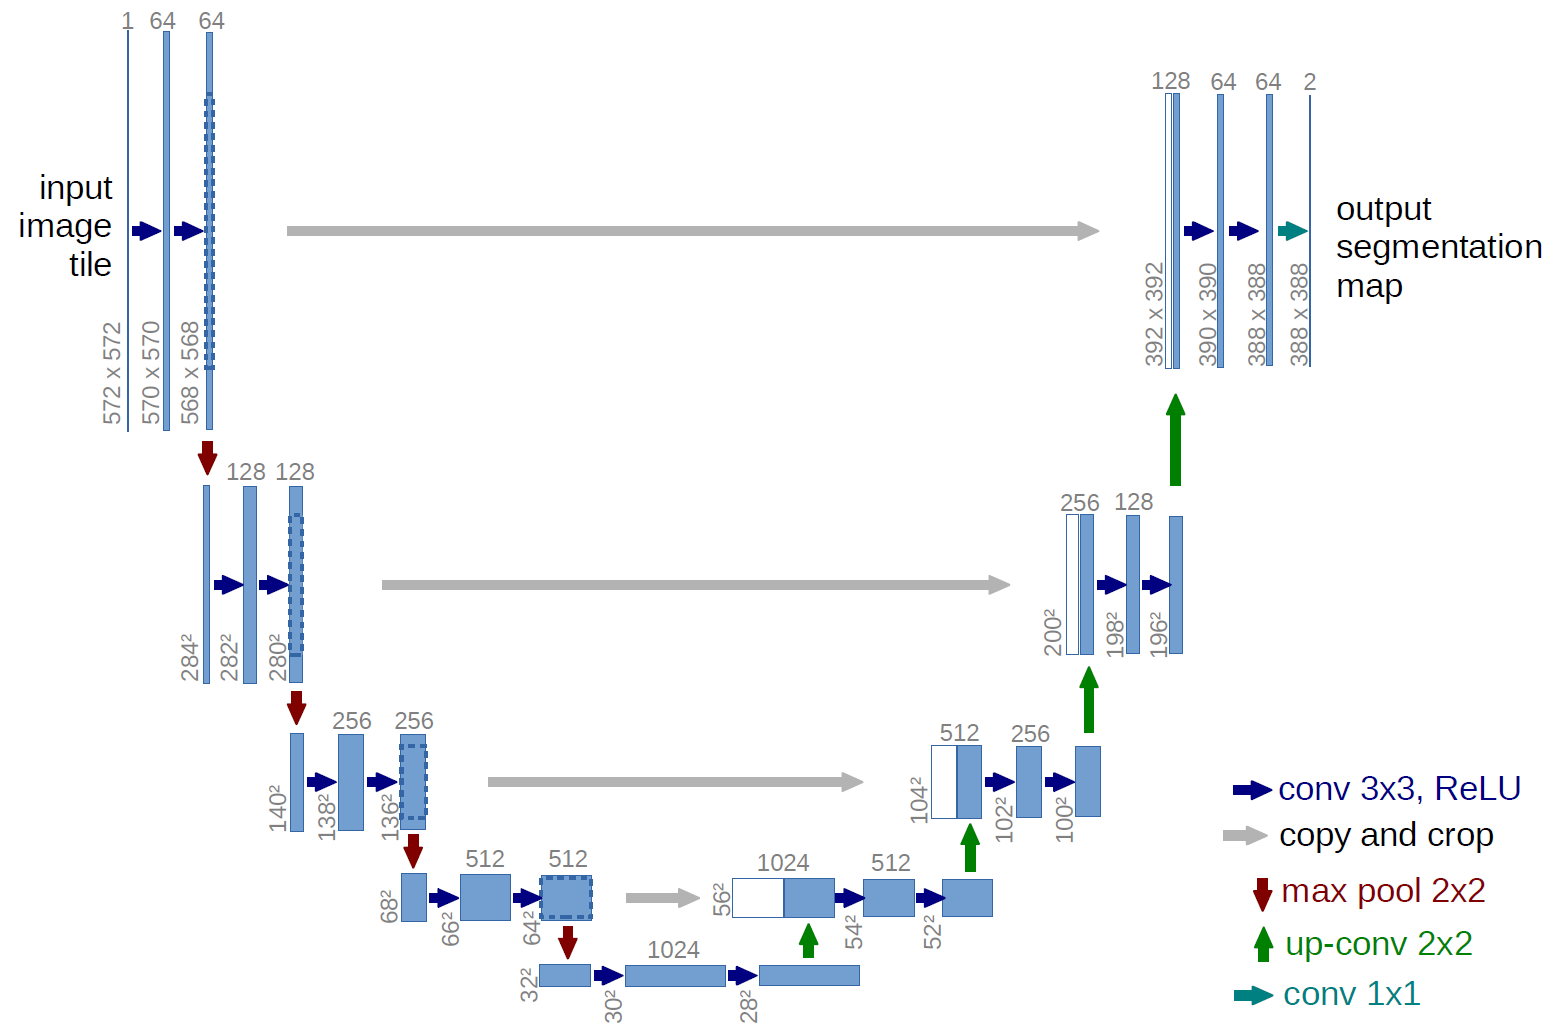
\includegraphics[width=0.6\paperwidth]{u-net-architecture}

\caption{Original u-net architecture, as seen in the original paper \citep{unet}.
Arrows represent operations between the multi-channel feature maps
represented by the rectangles. The number on top of each rectangle
is its number of channels and the numbers in the lower-left corner
are the $x$ and $y$ dimensions of the feature maps.}
\label{fig:unet-architecture}
\end{figure*}
\citet{unet} introduced the U-net architecture, a novel CNN architecture
that won several biomedical image segmentation challenges. Since the
original implementation in Caffe \citep{caffe}, others have implemented
U-net in numerous other frameworks and systems\footnote{Numbers by \href{https://paperswithcode.com/paper/u-net-convolutional-networks-for-biomedical}{Papers with Code}
as of March, 2022.}, including PyTorch \citep{pytorch}. 

Figure \ref{fig:unet-architecture} shows the original diagram that
represents the U-net architecture \citep{unet}. The blue right arrows,
labeled “conv 3x3, ReLU”, represent unpadded convolutions with
$3\times3$ kernels. After each of these convolutions, the size of
the feature map decreases by $2$, from which it can be inferred that
the stride \citep{conv-arithmetic-guide} is $1$. A rectified linear
unit (ReLU) \citep{relu} activation function follows each convolution.
After two such convolutions, max-pooling operations represented by
the red down arrows downsample each feature map to half the size using
a $2\times2$ region with stride $2$.\footnote{This makes the input size somewhat brittle. Specifically, the input
dimensions must be congruent to $12\mod16$} After every downsampling step, the first convolution doubles the
number of channels. The pattern of two convolutions (with ReLUs) followed
by downsampling via max-pooling happens four times and makes up the
contracting path of the network, on the left of the diagram.

After the contracting path (at the diagram bottom) completes, a corresponding
expanding path reduces the channels while increasing the map size.
Expansion uses unpadded $3\times3$ convolutions preceded by an upsampling
operation (green up arrows) that doubles the map size while halving
the channels. We infer that the original authors used a transposed
convolution (with $2\times2$ kernels) of stride $2$ \citep{conv-arithmetic-guide}\footnote{See \citep{up-transposed} for an informal discussion of this inference.}.
Half of the channels to the initial convolution after upsampling come
from the corresponding map on the contracting side of the architecture,
as represented by the gray right long arrows in the middle of the
diagram. The copied maps are center cropped to ensure matching dimensions.
At the end of the contracting path, a $1\times1$ unpadded convolution
reduces the $64$ feature maps to $2$ feature maps (one per class).

\subsection{APL Notation}

APL, introduced by Turing award winner Kenneth E. Iverson in the '60s
\citep{apl}, is an executable mathematical notation \citep{apl-since-78}.
This section introduces the basics of the notation used in this paper,
but \citet{mdapl} more fully describes the language. Online interactive
systems allow for experimentation with the language without needing
to install anything.\footnote{\url{https://tryapl.org}} All notation
used here is compatible with Dyalog APL 18.0\footnote{\url{https://dyalog.com/}}.

\subsubsection{Arrays}

\begin{table}
\caption{Array names according to \emph{rank}.\label{tab:rank-names}}
\begin{tabular}{ll}
\emph{Rank} & \emph{Name}\tabularnewline
\midrule 
0 & Scalar\tabularnewline
1 & Vector\tabularnewline
2 & Matrix\tabularnewline
3 & Cuboid\tabularnewline
4 & Hypercube\tabularnewline
5+ & Noble\tabularnewline
\bottomrule
\end{tabular}
\end{table}

The primary datatype of an APL system is the array.\footnote{Other types may exist for commercial systems, but these are not treated
here.} In APL, an array is an $N$-dimensional rectangular arrangement of
one or more elements in row-major order according to a list of zero
or more orthogonal dimensions (axes) called its \noun{shape}, with
the number of axes called its \noun{rank}. Table \ref{tab:rank-names}
gives the common names for sub-classes of arrays by rank. Scalars
have exactly one element. Higher ranked, non-empty arrays contain
as many elements as the product of its axes, while those with at least
one zero length axis, called \noun{empty} arrays, have a single element
called the \noun{prototype}, or \noun{fill}, element. For all numeric
arrays, such as those used in this paper, the fill element is \texttt{0},
and it is used by some primitives to extend or resize arrays to larger
shapes. Indices begin at 0, rather than 1.\footnote{Dyalog APL defaults to 1-based indexing.}

The elements of an array consist solely of other arrays, allowing
APL to have a single, uniform datatype.\footnote{This historically contentious design choice will be taken for granted.
Industrious readers may explore alternative designs elsewhere.} To make computation meaningful, APL defines a set of scalar arrays
that correspond to primitive values in the system, such as numbers
and characters. Thus, when we write a number like \texttt{1}, \texttt{3.5},
or \texttt{1e¯8}, this is the scalar array corresponding to that number
in the APL system.

\subsubsection{Expressions}

Expressions consist of a series of literals/variables, applications,
bindings, or assignments. Literal expressions describe an array. A
single numeric value is a literal. Adjacent values, separated by whitespace,
form a vector of those values. For example:
\begin{verbatim}
¯5    ⍝ Scalar negative 5
5 3 1 ⍝ Vector of 3 elements
\end{verbatim}
Note the use of a high minus to indicate a literal negative number
instead of \texttt{-5}, which is the application of the negate function
to \texttt{5}.

Functions can be first or second order. First order functions, called
\noun{functions}, take arrays as arguments and return a single array
value as a result, while second order functions, called \noun{operators,
}take arrays or \noun{functions} as arguments and return a \noun{function
}result. From now on, we use the term \noun{function} to refer to
first-order functions only. Application takes one of the following
infix forms:
\begin{verbatim}
   fn ⍵  ⍝ Monadic function application
 ⍺ fn ⍵  ⍝ Dyadic  function application
⍺⍺ op    ⍝ Monadic operator application
⍺⍺ op ⍵⍵ ⍝ Dyadic  operator application
\end{verbatim}
The terms \noun{monadic} and \noun{dyadic} refer to arity, not monads
in the functional programming sense. We use \texttt{⍺}, \texttt{⍵},
\texttt{⍺⍺}, and \texttt{⍵⍵} to refer to the left and right arguments
(for function application) and operands (for operator application),
respectively. Operators have higher binding precedence than functions,
and operators always associate to the left while functions always
associate to the right. This applies even in cases where traditional
math primitives are used. Consider the following example, where \texttt{⌿}
is a monadic operator, and \texttt{.} a dyadic:
\begin{verbatim}
   +.×⌿-2×3-4+3×5
←→ (((+.×)⌿)(-(2×(3-(4+(3×5))))))
\end{verbatim}
Notice that \texttt{-} is applied both monadically and dyadically. 

\subsubsection{Primitives}

APL is known for its primitives: built-in functions and operators
assigned special symbols instead of the standard alphanumeric variable
names given to user-defined values. The examples used in this paper
are expressions of mostly primitive functions and operators.

The largest class of primitives are the \noun{scalar functions}, defined
over a single scalar value or values and extended to all arrays by
point-wise, also called element-wise, extension. The left and right
arguments of a scalar function must share the same shape, with scalar
arguments extended to the same shape as the other argument. Consider
the following example using addition:
\begin{verbatim}
      5+1 3 7 10 ⍝ Scalar extension
6 8 12 15
\end{verbatim}
Scalar functions return arrays the same shape as their inputs. The
set of scalar functions used in this paper include the standard arithmetic
functions \texttt{+}, \texttt{×}, \texttt{÷}, \texttt{-}, \texttt{⌈}
(ceiling or maximum), \texttt{⌊} (floor/minimum), \texttt{|} (absolute
value), and \texttt{{*}} (exponent), as well as the Boolean relations
\texttt{<}, \texttt{≤}, \texttt{=}, \texttt{≠}, \texttt{≥}, \texttt{>},
and \texttt{\textasciitilde} (not) which return \texttt{1} for \noun{true}
and \texttt{0} for \noun{false}.

The core primitive \texttt{⍴} is used for the shape of an array. The
monadic application \texttt{⍴⍵} returns a vector of the axes of \texttt{⍵}.
The dyadic application \texttt{⍺⍴⍵} returns an array whose shape is
\texttt{⍺} and whose elements are taken in wrapping order from \texttt{⍵}.
For example:
\begin{verbatim}
      3 5⍴1 2 3 4 ⍝ A 3×5 matrix
1 2 3 4 1
2 3 4 1 2
3 4 1 2 3
\end{verbatim}
The function \texttt{≢⍵} applied monadically returns the length of
the first axis of \texttt{⍵}, that is, the first element of \texttt{⍴⍵}. 
\begin{verbatim}
      ≢7 5 6⍴0
7
\end{verbatim}
Thus, the rank of an array is given by \texttt{≢⍴⍵}.
\begin{verbatim}
      ≢⍴7 5 6⍴0
3
\end{verbatim}
The expression \texttt{⍳N} gives the natural numbers up to \texttt{N}.
\begin{verbatim}
      ⍳7
0 1 2 3 4 5 6
\end{verbatim}
The primitives \texttt{⊖} and \texttt{⌽} rotate arrays along the first
and last axis, respectively. Applied monadically, they reverse/flip
an array along the appropriate axis. When applied dyadically, they
shift an array by the specified amount. Thus \texttt{¯2⌽⍵} rotates
(with wrapping) \texttt{⍵} two positions to the right along the last
axis. Writing \texttt{⌽{[}x{]}} or \texttt{⊖{[}x{]}}specifies rotation
along axis \texttt{x}. 
\begin{verbatim}
      ¯1⊖3 5⍴1 2 3 4 ⍝ Shift down 1 row
3 4 1 2 3
1 2 3 4 1
2 3 4 1 2
\end{verbatim}
The transpose primitive \texttt{⍉} permutes its argument's axes into
different positions. Monadic \texttt{⍉⍵} reverses the shape of \texttt{⍵},
while giving \texttt{⍉} a left argument indicates how to permute the
dimensions. Thus, \texttt{0 1 3 2⍉⍵} transposes a hypercube \texttt{⍵}
by exchanging the last two axes; likewise, \texttt{3 0 1 2⍉⍵} transposes
\texttt{⍵} so that its first axis becomes its last, while all other
dimensions retain the same relative order. The following transposes
two matrix slices (sub-arrays) of a cube:
\begin{verbatim}
      2 3 3⍴0 1 2 3 4
0 1 2
3 4 0
1 2 3
     
4 0 1
2 3 4
0 1 2
      0 2 1⍉2 3 3⍴0 1 2 3 4
0 3 1
1 4 2
2 0 3
     
4 2 0
0 3 1
1 4 2
\end{verbatim}
The functions \texttt{↑} and \texttt{↓} resize \texttt{⍵} by taking
or dropping elements. The expression \texttt{2 ¯3↑⍵} will give a \texttt{2×3}
matrix from \texttt{⍵} with rows taken from the top and columns taken
from the right, since a negative size takes from the tail instead
of the head. Drop (\texttt{↓}) works the same way, but eliminates
instead of taking items. The following example centers a \texttt{2×2}
matrix into a \texttt{4×4} matrix. Notice how the matrix is extended
using \texttt{0} as the \noun{fill} element.
\begin{verbatim}
      2 2⍴1 2 3 4
1 2
3 4
      3 3↑2 2⍴1 2 3 4
1 2 0
3 4 0
0 0 0
      ¯4 ¯4↑3 3↑2 2⍴1 2 3 4
0 0 0 0
0 1 2 0
0 3 4 0
0 0 0 0
\end{verbatim}
The expression \texttt{⍺,⍵} catenates \texttt{⍺} and \texttt{⍵} together
as a single array along the last axis. However, in this paper we primarily
use \texttt{,} monadically. The expression \texttt{,⍵} gives a vector
of the elements of \texttt{⍵}, collapsing the axes of \texttt{⍵} into
a single axis whose size is the product of the axes of \texttt{⍵}.
We write \texttt{,{[}d{]}⍵} to collapse the specified axes \texttt{d}
to a single axis. The following example collapses the trailing two
axes of a cube, creating a matrix:
\begin{verbatim}
      2 3 3⍴0 1 2 3 4
0 1 2
3 4 0
1 2 3
     
4 0 1
2 3 4
0 1 2
      ,[1 2]2 3 3⍴0 1 2 3 4
0 1 2 3 4 0 1 2 3
4 0 1 2 3 4 0 1 2
\end{verbatim}
We write \texttt{N⌿⍵} or \texttt{N/⍵} to mean the array \texttt{⍵}
with each element duplicated \texttt{N} times along the first or last
axis, respectively:
\begin{verbatim}
      2 2⍴1 2 3 4
1 2
3 4
      2⌿2/2 2⍴1 2 3 4
1 1 2 2
1 1 2 2
3 3 4 4
3 3 4 4
\end{verbatim}
The expressions \texttt{f⌿⍵} and \texttt{f/⍵} compute the reduction
of \texttt{⍵} using function \texttt{f} over the first or last axis,
respectively. This is often called a right fold in many functional
languages.
\begin{verbatim}
      +⌿1 2 3 4 5
15
\end{verbatim}
The dyadic application \texttt{+.×} is the function for matrix multiplication
extended to higher dimensions. 

We can mutate the elements of an array or bind the result of an expression
to a name. The form \texttt{V←expr} binds \texttt{V} to the result
of \texttt{expr}. The expression \texttt{A{[}i{]}}←\texttt{expr} assigns
the elements of \texttt{expr} to the corresponding elements of \texttt{A}
according to indices \texttt{i}. If we have a nested array \texttt{A}
in which we want to store a single non-scalar array \texttt{X} at
index \texttt{i}, we box the value \texttt{X} into a scalar first,
using \texttt{⊂}, resulting in the expression \texttt{A{[}i{]}←⊂X}.
We write \texttt{i⊃A} to extract the same array \texttt{X} from \texttt{A}.

The syntax \texttt{\{expr+ ...\}} returns a function. Within the body
of the function, consisting of a set of expressions, \texttt{⍺} is
the left argument to the function and \texttt{⍵} is the right, while
\texttt{∇} refers to the function itself, permitting anonymous recursion.
Functions execute expressions in order and return the first unbound
expression or the last bound expression.
\begin{verbatim}
      add1←{1+⍵}
      add1 3 4 5
4 5 6
\end{verbatim}

\section{Implementation}

\subsection{Overview}

Our implementation of U-net divides into two significant considerations:
the implementation of the fundamental vocabulary of neural networks
and the wiring of those operations into the actual U-net architecture.
We leverage features of APL to implement both aspects of the system,
and so we treat each in its own sub-section. 

Because Co-dfns does not yet support the complete array of Dyalog
primitives and their semantics, we could enhance some implementation
techniques through the use of the richer feature-set. The effect of
these features would be increased concision and clarity, but such
improvements would not significantly affect the overall performance
of the code, either positively or negatively. The overall structure
of the code is clear and simple enough in its current state to warrant
inclusion almost verbatim, but some adjustments were made to reduce
the total number of primitives used, which makes the code slightly
less elegant while reducing the burden to the reader to learn more
APL primitives.

One area deserving particular attention is the design of APL as a
language itself and the features that present themselves as well-suited
to expressing neural network computations. Our exploration of these
features uncovered design tensions worth discussing in detail. A complete
copy of the code discussed in this paper is included in the appendices.

\subsection{Design of APL Primitives for Neural Networks}

The majority of APL primitives find fundamental use in computing neural
networks, which isn't surprising given the array-oriented and numerical
nature of the domain. However, the stencil operator, introduced in
Dyalog APL \citep{stencil-lives}, stands out as the most obviously
aligned with convolutional neural networks. The J programming language
introduced an alternative implementation of the stencil operator earlier
\citep{stencil-in-J}, from which Dyalog derived inspiration for the
implementation of their own stencil operator. We propose an alternative
that was first suggested to us by the late Roger Hui, the stencil
\noun{function} \citep{SF-hui-blog}. The stencil function is a function
whose left argument is the same as the right operand of the stencil
operator, and which receives the same right argument as the right
argument to the function returned by the stencil operator. A reasonable
definition (padded) of the stencil function using the Dyalog stencil
operator might be:
\begin{verbatim}
SF←{({⍵}⌺⍺)⍵}
\end{verbatim}
A naïve implementation of the stencil function that did not pad its
results was implemented in Co-dfns and used in U-net implementation.
We subsequently use \texttt{⌺} to mean the stencil \noun{function}
without padding and not the stencil \noun{operator} as it appears
in Dyalog APL. Given a specification \texttt{s} as the left argument,
the stencil function, written \texttt{s⌺a}, returns an array of each
sliding window slice of \texttt{a} specified by \texttt{s}. The first
row of the specification indicates the window sizes while the second
row indicates the step size, or 1 if omitted. The window is conceptually
“slid” along the leading axes of the input array. The two most
common sliding window sizes for \texttt{⌺} in U-net are \texttt{3
3} for convolutions, corresponding to a window size of \texttt{3×3}
and a step of \texttt{1} for each axis, and \texttt{2 2⍴2} (a 2 by
2 matrix of 2's) for the max pooling layers and up convolutions, corresponding
to a \texttt{2×2} window size and a step of \texttt{2} for each axis.

For example, a \texttt{3 3} sliding window of step 1 on a \texttt{6
6} matrix returns an array of shape \texttt{4 4 3 3} consisting of
16 \texttt{3 3} matrix slices arranged in a \texttt{4 4} grid. The
dimensions of the two leading axes will shrink by 2 each time because
we implemented stencil without padding.
\begin{verbatim}
      6 6⍴⍳36
 0  1  2  3  4  5
 6  7  8  9 10 11
12 13 14 15 16 17
18 19 20 21 22 23
24 25 26 27 28 29
30 31 32 33 34 35
      ⍴3 3⌺6 6⍴⍳36
4 4 3 3
\end{verbatim}
In the following, we box each \texttt{3 3} matrix slice using \texttt{⊂{[}2
3{]}} to show the slices in a more compact form as a nested matrix
of matrices, but the result of \texttt{⌺} is actually a rank 4 hypercube
in this case.
\begin{verbatim}
      ⊂[2 3]3 3⌺6 6⍴⍳36
┌────────┬────────┬────────┬────────┐
│ 0  1  2│ 1  2  3│ 2  3  4│ 3  4  5│
│ 6  7  8│ 7  8  9│ 8  9 10│ 9 10 11│
│12 13 14│13 14 15│14 15 16│15 16 17│
├────────┼────────┼────────┼────────┤
│ 6  7  8│ 7  8  9│ 8  9 10│ 9 10 11│
│12 13 14│13 14 15│14 15 16│15 16 17│
│18 19 20│19 20 21│20 21 22│21 22 23│
├────────┼────────┼────────┼────────┤
│12 13 14│13 14 15│14 15 16│15 16 17│
│18 19 20│19 20 21│20 21 22│21 22 23│
│24 25 26│25 26 27│26 27 28│27 28 29│
├────────┼────────┼────────┼────────┤
│18 19 20│19 20 21│20 21 22│21 22 23│
│24 25 26│25 26 27│26 27 28│27 28 29│
│30 31 32│31 32 33│32 33 34│33 34 35│
└────────┴────────┴────────┴────────┘
\end{verbatim}
Notice that the window slides along the leading axes, so each slice
captures all trailing axes for each slice.

\subsection{Neural Network Vocabulary\label{subsec:Neural-Network-Vocabulary}}

The original U-net paper uses five distinct operations to describe
the network (see \prettyref{fig:unet-architecture}):
\begin{enumerate}
\item A \texttt{3×3} convolution with a ReLU activation function is used
as the primary operation
\item A copy and crop operation is used to transfer data across one row
of the network
\item Max pooling layers on a \texttt{2×2} window are used to compute “down”
the network
\item A \texttt{2×2} transposed convolution goes back “up” the network
\item The final output has a single \texttt{1×1} convolution with a soft-max
layer
\end{enumerate}
In our implementation, we mirror this vocabulary by implementing the
forward and back functions for each of these layers, one for each
of the above operations. This results in a total of 10 functions grouped
into 5 pairs, which we will take in turn.

Each of our operations works over a given network “layer,” which
is a cube of shape \texttt{N M C} where \texttt{N M} are the layer
dimensions and \texttt{C} is the number of layer channels. 

\subsubsection{Convolution (3×3) with ReLU}

The primary U-net convolutional kernel is a 3×3 convolution with a
ReLU activation function. The convolution in the paper uses “valid”
convolutions, meaning that no padding is used. This implies that the
convolution dimensions of the output array shrink by 2 for each dimension
compared to the input. We define the forward propagation function
\texttt{CV} as a function over a kernel \texttt{⍺} of shape \texttt{3
3 I O} of \texttt{I} input channels and \texttt{O} output channels
with a layer \texttt{⍵} of shape \texttt{N M I} that obeys the following
shape invariant:
\begin{verbatim}
⍴⍺ CV ⍵ ←→ (¯2+2↑⍴⍵),¯1↑⍴⍺
\end{verbatim}
This says that the size of the first two axes of \texttt{⍺ CV ⍵} will
be two less than the first two axes of \texttt{⍵}, while the remaining
axis, corresponding to the output channels, will match the last axis
of \texttt{⍺}. In other words, given the kernel of shape \texttt{3
3 I O} and layer of shape \texttt{N M I}, the result of \texttt{⍺
CV ⍵} will have shape \texttt{(N-2) (M-2) O}. Using the stencil function,
we define \texttt{CV} as follows for rank 4 kernel inputs and rank
3 layer inputs:
\begin{verbatim}
CV←{0⌈(,[2 3 4]3 3⌺⍵)+.×,[0 1 2]⍺}
\end{verbatim}
The result of the expression \texttt{3 3⌺⍵} will have a rank of 5
and shape \texttt{(N-2) (M-2) 3 3 I}, so raveling the trailing dimensions
with the expression \texttt{,{[}2 3 4{]}3 3⌺⍵} gives us a cube of
shape \texttt{(N-2) (M-2) (3×3×I)} while the expression \texttt{,{[}0
1 2{]}⍺} gives us a matrix of shape \texttt{(3×3×I) O}. We use the
extended matrix multiplication \texttt{+.×} to compute the convolution,
resulting in a cube of shape \texttt{N M O}. The ReLU function \texttt{0⌈⍵}
follows as the final operation. 

Computing backpropagation uses very similar approaches. Given the
output layer \texttt{z}, input layer \texttt{x}, activation layer
\texttt{a}, weights \texttt{⍺}, and the gradient backpropagated so
far \texttt{⍵}, we compute the transposed weights \texttt{w}, the
derivative output layer \texttt{∆z}, the weight gradient \texttt{∆w},
padded output layer \texttt{∆Z}, and the resulting back gradient \texttt{∆x}
as follows:
\begin{verbatim}
∆CV←{
     w←⊖⌽[1]0 1 3 2⍉⍺
    ∆z←⍵×0<a
    ∆w←3 0 1 2⍉(⍉,[0 1]∆z)+.×,[0 1]3 3⌺x
    ∆Z←¯2⊖¯2⌽[1](4+2↑⍴∆z)↑∆z
    ∆x←(,[2 3 4]3 3⌺∆Z)+.×,[0 1 2]w
}
\end{verbatim}
Since our stencil function does not pad its results, the expression
\texttt{¯2⊖¯2⌽{[}1{]}(4+2↑⍴∆z)↑∆z} expands the shape of \texttt{∆z}
to ensure that the output convolution dimensions are 2 greater than
those of \texttt{∆z}.

\subsubsection{Copy and Crop}

Conceptually, the copy and crop operation is the simplest of the functions
in U-net. Its sole job is to take the output from one side of the
U-shaped net and move it over to the other side, adjusting the dimensions
to ensure that it fits. In the forward direction, the input layer
will have a greater dimension than the output layer, so we crop as
evenly as possible around the edges and then catenate the result at
the head of the layer coming “up” from the network to form the
output layer with twice the channels of the “up” layer. The
following function \texttt{CC} computes the crop of \texttt{⍺} catenated
with \texttt{⍵} using \texttt{↓}:
\begin{verbatim}
CC←{
    p←((⍴⍺)-⍴⍵)÷2),⍵
    ((⌊p)↓(-⌈p)↓⍺
}
\end{verbatim}
For dimensions not evenly divisible by two, we choose to round up
on the right and bottom sides and round down on the left and upper
sides of the layer. Computing the backpropagation of \texttt{CC} given
the input \texttt{⍺} and output gradient \texttt{⍵} simply reverses
this operation and expands the shape back to the original input size.
This result is then added to the appropriate layer in the U-net architecture
described in \prettyref{subsec:U-net-Architecture}. 
\begin{verbatim}
∆CC←{
    n m←-⌊(2↑(⍴⍺)-⍴⍵)÷2
    ∆x←n⊖m⌽[1](⍴⍺)↑⍵
}
\end{verbatim}

\subsubsection{Max Pooling}

Max pooling is a shrinking convolution that computes the maximum value
in a non-overlapping sliding window. Given the stencil function, the
max pool over a layer is given by the following definition for \texttt{MX}:
\begin{verbatim}
MX←{⌈⌿[2],[2 3](2 2⍴2)⌺⍵}
\end{verbatim}
Here we write \texttt{⌈⌿{[}2{]},{[}2 3{]}⍵} to describe an array where
we have collapsed dimensions 2 and 3 and computed the maximum value
reduction over the resulting dimension. For example, given an input
layer \texttt{⍵} of shape \texttt{N M C}, the result of \texttt{(2
2⍴2)⌺⍵} is a rank 5 array of shape \texttt{(N÷2) (M÷2) 2 2 C}. We
then collapse axes 2 and 3 to form an array of shape \texttt{(N÷2)
(M÷2) 4 C} and subsequently find the maximum value for each vector
along axis 2, resulting in an array of shape \texttt{(N÷2) (M÷2) C}.

Computing the backpropagation of this involves replicating each of
the stencil dimensions, which are the two leading axes in our implementation.
Given an input \texttt{⍺} and output layer \texttt{⍵} the following
function \texttt{∆MX} computes the backpropagation:
\begin{verbatim}
∆MX←{
    y←(⍴⍺)↑2⌿2/[1]⍵
    y×⍺=y
}
\end{verbatim}

\subsubsection{Transposed Convolution (2×2)}

The upsampling computation with convolution proved to be the most
subtle and challenging, mostly due to the opaqueness of implementations.
The U-net paper was not immediately transparent regarding the exact
operations used for this layer and there were a number of potential
design decisions that could have been made. Moreover, for users reading
about upsampling through convolutions, the descriptions are also the
furthest removed from a reasonable implementation of the same. However,
once the intuition hits that an upsampling convolution matches the
shape and form of a non-overlapping sliding window in the output layer,
the computation becomes much clearer.\footnote{\href{https://mathspp.com/blog/til/033}{https://mathspp.com/blog/til/033}}

For this convolution, we change the anticipated kernel shape from
that used for \texttt{CV} above. Whereas \texttt{CV} expects kernels
of shape \texttt{3 3 I O}, our transposed convolutions expect kernels
of shape \texttt{I 2 2 O} for input channels \texttt{I} and output
channels \texttt{O}. With a layer of standard shape \texttt{N M I},
this gives the following definition for the upsampling pass:
\begin{verbatim}
UP←{,[0 1],[2 3]0 2 1 3 4⍉⍵+.×⍺}
\end{verbatim}
The key change here from the reliance on \texttt{+.×} with \texttt{CV}
is the use of a dyadic transpose. The input into the \texttt{⍉} transpose
is the result of \texttt{⍵+.×⍺} which has shape \texttt{N M 2 2 O}.
Thus, the expression \texttt{0 2 1 3 4⍉⍵+.×⍺} returns an array of
shape \texttt{N 2 M 2 O}. As the final operation, we collapse the
first two pairs of leading dimensions, giving a final output array
of shape \texttt{(N×2) (M×2) O}. 

To compute the backpropagation pass, we compute the convolutions on
a \texttt{2×2} sliding window with stride 2.
\begin{verbatim}
∆UP←{
    ∆w←(⍉,[0 1]x)+.×,[0 1](2 2⍴2)⌺∆z
    ∆x←(,[2 3 4](2 2⍴2)⌺∆z)+.×⍉,[1 2 3]⍺
}
\end{verbatim}

\subsubsection{Final 1×1 Convolution}

The final convolution is a \texttt{1×1} convolution with 2 output
channels, which means that it collapses the final incoming channels
into an output layer with only two channels. This gives the trivial
simplification of our convolution code over layer \texttt{⍵} and kernel
\texttt{⍺} of \texttt{⍵+.×⍺}, which we combine with the soft-max layer
described in the paper:
\begin{verbatim}
C1←{
    z←⍵+.×⍺
    z←*z-[0 1]⌈/z
    1E¯8+z÷[0 1] +/z
}
\end{verbatim}
Computing the backpropagation is likewise a simplification of the
more complex \texttt{CV} code:
\begin{verbatim}
∆C1←{
    ∆w←(⍉,[0 1]x)+.×,[0 1]∆z
    ∆x←∆z+.×⍉w
}
\end{verbatim}
\begin{table*}
\caption{A rectangular arrangement of the U-net network\label{tab:A-rectangular-arrangement}}

\begin{tabular}{crrrlrrrlrr}
 &  & \multicolumn{7}{c}{\noun{Operation}} &  & \tabularnewline
\cmidrule{3-9} \cmidrule{4-9} \cmidrule{5-9} \cmidrule{6-9} \cmidrule{7-9} \cmidrule{8-9} \cmidrule{9-9} 
 &  & \multicolumn{1}{l}{$CV$} & \multicolumn{1}{l}{$CV$} & $MX$ &  & \multicolumn{1}{l}{$CV$} & \multicolumn{1}{l}{$CV$} & $UP$ &  & \tabularnewline
\cmidrule{3-5} \cmidrule{4-5} \cmidrule{5-5} \cmidrule{7-9} \cmidrule{8-9} \cmidrule{9-9} 
\multirow{4}{*}{\begin{turn}{90}
\noun{Depth}
\end{turn}} & {\tiny{}0} & \texttt{\tiny{}$\texttt{3\ 3\ \ \ 1\ \ 64}$} & {\tiny{}$\texttt{3 3 \ 64 \ 64}$} & {\tiny{}$\texttt{0 0 \ 64 \ 64}$} &  & {\tiny{}$\texttt{3 3 \ 256 \ 128}$} & {\tiny{}$\texttt{3 3 \ 128 \ 128}$} & {\tiny{}$\texttt{\ 128 2 2 \ 64}$} &  & \tabularnewline
 & {\tiny{}1} & \multirow{1}{*}{{\tiny{}$\texttt{3\ 3\ \ 64\ 128}$}} & {\tiny{}$\texttt{3 3 128 128}$} & {\tiny{}$\texttt{0 0 128 128}$} &  & {\tiny{}$\texttt{3 3 \ 512 \ 256}$} & {\tiny{}$\texttt{3 3 \ 256 \ 256}$} & {\tiny{}$\texttt{\ 256 2 2 128}$} &  & \tabularnewline
 & {\tiny{}2} & {\tiny{}$\texttt{3 3 128 256}$} & {\tiny{}$\texttt{3 3 256 256}$} & {\tiny{}$\texttt{0 0 256 256}$} &  & {\tiny{}$\texttt{3 3 1024 \ 512}$} & {\tiny{}$\texttt{3 3 \ 512 \ 512}$} & {\tiny{}$\texttt{\ 512 2 2 256}$} &  & \tabularnewline
 & {\tiny{}3} & {\tiny{}$\texttt{3 3 256 512}$} & {\tiny{}$\texttt{3 3 512 512}$} & {\tiny{}$\texttt{0 0 512 512}$} &  & {\tiny{}$\texttt{3 3 \ 512 1024}$} & {\tiny{}$\texttt{3 3 1024 1024}$} & {\tiny{}$\texttt{1024 2 2 512}$} &  & \tabularnewline
\cmidrule{3-5} \cmidrule{4-5} \cmidrule{5-5} \cmidrule{7-9} \cmidrule{8-9} \cmidrule{9-9} 
 &  & \multicolumn{3}{c}{\emph{Downward Pass}} &  & \multicolumn{3}{c}{\emph{Upward Pass}} &  & \tabularnewline
\cmidrule{3-5} \cmidrule{4-5} \cmidrule{5-5} \cmidrule{7-9} \cmidrule{8-9} \cmidrule{9-9} 
\end{tabular}
\end{table*}


\subsection{U-Net Architecture\label{subsec:U-net-Architecture}}

Given the core vocabularies defined in \prettyref{subsec:Neural-Network-Vocabulary},
the remaining challenge with implementing U-net is to link together
the appropriate layers and compositions to form the complete network
as described by \prettyref{fig:unet-architecture}. To do this, we
observe that the structure of the U-net diagram is an almost symmetric
pattern. The output layer computations form three operations which
are not part of the pattern, but the rest of the pattern decomposes
into 4 depths, each with 6 operations each. \prettyref{tab:A-rectangular-arrangement}
contains a visual arrangement of the kernel shapes used in our architecture
mirroring the overall structure of \prettyref{fig:unet-architecture}. 

Additionally, we note that the U-shaped structure also mimics the
down and up nature of a recursive program call-tree. Thus, our overall
strategy is to implement a recursive function \texttt{LA} that receives
an index identifying a particular depth of the network, computes the
appropriate “downward pass” operations before recurring deeper
into the network and finally computing the upwards passes on the return
of its recursive call. We likewise implement backpropagation in same
way, but in the opposite direction. Assuming that \texttt{⍺} contains
the computed depth offset for the network layer, we write \texttt{⍺+i}
to access the $i$th column of the network described in \prettyref{tab:A-rectangular-arrangement}
at the depth \texttt{⍺÷6}. 

Our architecture is agnostic to any specific size of kernels or depth
of the “U”; using greater depth with larger resolutions is possible
simply by providing a different network of kernels as input. Many
systems typically allocate networks statically, including our own
PyTorch implementation. Our implementation instead assumes a network
defined by a set of kernels \texttt{W} that match the expected shape.
We mirror the \texttt{W} network with our intermediate results in
\texttt{Z} so that we can do backpropagation. The full code for our
layers extract their values from these \texttt{Z} and \texttt{W} vectors
directly using expressions like \texttt{⍺⊃W} to extract the weights
for the layer at index \texttt{⍺}. We likewise store intermediate
results with expressions like \texttt{Z{[}⍺{]}←⊂⍵}.

Our forward pass function is responsible for initializing \texttt{Z}
to hold the intermediate results produced by forward propagation for
use by the backpropagation function. After the recursive computation,
there are the final three operations, \texttt{C1} and two \texttt{CV}
operations, that must be called before returning. We assume that we
may receive a rank 2 matrix instead of a rank 3 layer as input, and
so we reshape the input to ensure that we always have a rank 3 input
to \texttt{LA}. This gives us the following function definition:
\begin{verbatim}
FWD←{
  Z⊢←(≢W)⍴⊂⍬
  ⍝ Forward propagation layers ...
  LA←{
    ⍺≥≢Z:⍵
    down←(⍺+6)∇(⍺+2)MX(⍺+1)CV(⍺+0)CV ⍵
    (⍺+2)CC(⍺+5)UP(⍺+4)CV(⍺+3)CV down
  }
  2 C1 1 CV 0 CV 3 LA (3↑(⍴⍵),1)⍴⍵
}
\end{verbatim}
The backwards computation mirrors this pattern, except that it proceeds
in the opposite direction and also defines an updater function \texttt{∆}
that will update the network weights in \texttt{W} and the velocities
in \texttt{V} based on a given gradient \texttt{⍵} and index \texttt{⍺}
pointing to a specific location in the network. 
\begin{verbatim}
BCK←{
  Y←⍺ ⋄ Y∆←⍵
  ∆←{
    V[⍺]←⊂⍵+MO×(⍴⍵)⍴⍺⊃V
    W[⍺]←⊂(⍺⊃W)-LR×⍺⊃V
  }
  ⍝ Back propagation layers ...
  ∆LA←{
    ⍺≥≢Z:⍵
    up←(⍺+5)∆UP(-(≢⍉⍵)÷2)↑[2]⍵
    down←(⍺+6)∇(⍺+3)∆CV(⍺+4)∆CV up
    mx←(⍺+2)∆MX down
    (⍺+0)∆CV(⍺+1)∆CV mx+(⍺+2)∆CC ⍵
  }
  diff←Y∆-(~Y),[1.5]Y
  3 ∆LA 0 ∆CV 1 ∆CV 2 ∆C1 diff
}
\end{verbatim}

\section{Performance}

We primarily focused on comparing our U-net implementation against
a reference implemented in PyTorch \citep{pytorch}, which is an easy
to use Python framework with good performance. 

\begin{figure*}
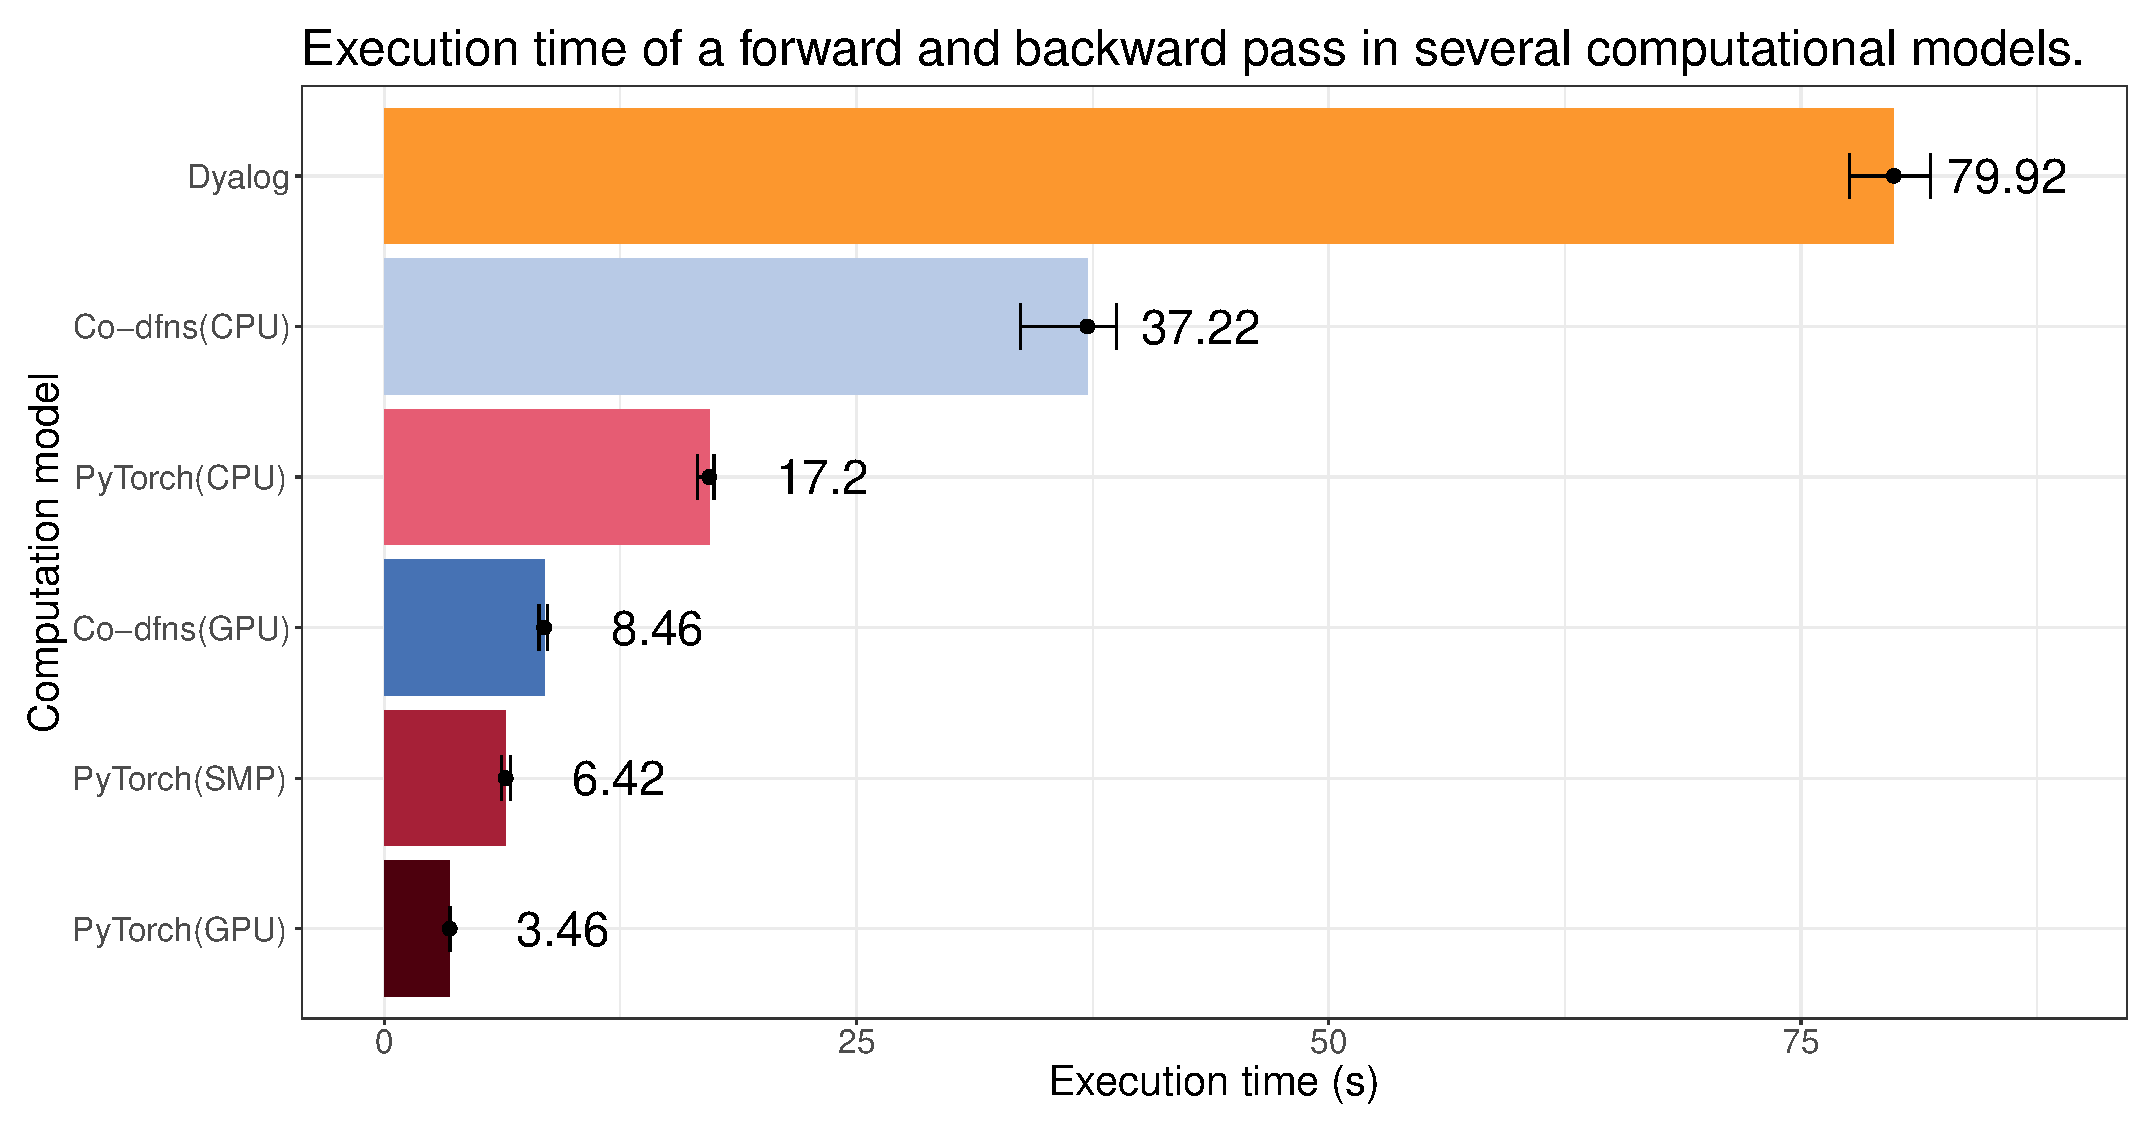
\includegraphics[width=1\textwidth]{benchmark-comp}

\caption{Performance results for U-net across a range of platforms\label{fig:Performance-results-for}}
\end{figure*}
We were primarily interested in the costs of executing a single run
of the U-net over a single image source in both the forwards and backwards
directions. We compared performance over the following platforms:
\begin{itemize}
\item Dyalog APL 18.0 64-bit Windows interpreter
\item Co-dfns (v4.1.0 master branch) using the CUDA backend (AF v3.8.1)
\item Co-dfns (v4.1.0 master branch) using the CPU backend (AF v3.8.1)
\item PyTorch v1.10.2 with the CUDA GPU backend
\item PyTorch v1.10.2 with the multi-threaded CPU backend
\item PyTorch v1.10.2 with the single-threaded CPU backend
\end{itemize}
The results of the execution can be seen in \prettyref{fig:Performance-results-for}.
The timings do not include the cost of reading the image data from
disk, but they do include the costs of transferring the image input
data and the resulting error and forward propagation results back
to the CPU main memory. In our testing, data transfer costs in Co-dfns
accounted for significantly less than 5\% of the total runtime. 

The hardware used was an NVIDIA GeForce RTX 3070 Laptop GPU with 8GB
of dedicated graphics memory. We used NVIDIA driver version 511.65.
The CPU was an Intel Core i7-10870H with 16 logical cores @ 2.2GHz.
Main system memory was 32GB of DDR4 RAM. The system was running an
up to date release of Microsoft Windows 11. 

As input we used the original image data from the ISBI benchmark referenced
in the U-net paper \citep{unet,isbi-data}. These images are $512\times512$
images in grayscale with a binary mask for training. Each run took
one of these images and associated training mask and computed the
result of forward and backwards propagation and the error as well
as updating the weights for the network. 

When working on the network, APL implementations generally do not
have a concept of small floating point values. Rather, their default
is to always use 64-bit floating point values when floats are called
for. In order to try to mimic this behavior as closely as possible,
we attempted to feed 64-bit data into the PyTorch models. However,
because of the opaqueness of the PyTorch implementation, we were not
able to fully verify that 64-bit values are used throughout the PyTorch
computational network. On the other hand, the reliance on 64-bit only
floating points, while a boon to convenience and user-friendliness
for non-computer science programmers, creates well-defined performance
issues for an application like this.

When running the benchmark, we computed the average of 10 runs, ensuring
that we discarded the first run each time, since these runs often
contained significant setup and bootstrapping code (PyTorch's optimizer,
the JIT optimization in Co-dfns, and so forth). The figure includes
information about the variance of the individual runs as well as the
average run time in seconds. 

Examining the data, it is clear why traditional APL implementations
were relatively unsuited to extensive use within the machine learning
space. Dyalog's interpreter preformed the slowest by a very large
magnitude. After this, the single-threaded CPU implementations in
Co-dfns and PyTorch are predictably the next slowest, with the Co-dfns
implementation running about a factor of 2.2 times slower than the
equivalent PyTorch implementation.

When acceleration techniques are employed, the differences in execution
speed begin to shrink, with PyTorch's multi-threaded and GPU-based
implementations coming in fasted, and Co-dfns' GPU backend running
at roughly 2.4 times slower than the PyTorch GPU execution. 

We observed the widest variance in performance results in the Co-dfns
CPU and Dyalog interpreter-based runs, and very little variance in
the GPU-based runs or in PyTorch itself. 

The stencil function was modeled in APL and used to conduct the above
benchmark. The model, written in APL, is a naïve implementation of
the stencil function and contains no special optimizations other than
to distinguish between sliding windows of step 1 and non-overlapping,
adjacent windows (such as used for the max pooling layers). Additionally,
no specialized code was used within Co-dfns that was specific or specialized
to neural network programming. 

The above benchmark therefore represents a comparison of the PyTorch
implementation against a naïve and unspecialized implementation in
APL executed with the general-purpose runtime used in Co-dfns that
provides generalized GPU computation but does not include domain-specific
optimizations such as those available in PyTorch. 

\section{Discussion}

\subsection{Performance}

\begin{table*}
\caption{Raw Performance Timings (Secs)}

\centering{}%
\begin{tabular}{rr@{\extracolsep{0pt}.}lr@{\extracolsep{0pt}.}lr@{\extracolsep{0pt}.}lr@{\extracolsep{0pt}.}lr@{\extracolsep{0pt}.}lr@{\extracolsep{0pt}.}lr@{\extracolsep{0pt}.}lr@{\extracolsep{0pt}.}lr@{\extracolsep{0pt}.}lr@{\extracolsep{0pt}.}lr@{\extracolsep{0pt}.}lr@{\extracolsep{0pt}.}l}
 & \multicolumn{2}{c}{0} & \multicolumn{2}{c}{1} & \multicolumn{2}{c}{2} & \multicolumn{2}{c}{3} & \multicolumn{2}{c}{4} & \multicolumn{2}{c}{5} & \multicolumn{2}{c}{6} & \multicolumn{2}{c}{7} & \multicolumn{2}{c}{8} & \multicolumn{2}{c}{9} & \multicolumn{2}{c}{} & \multicolumn{2}{c}{\emph{Avg}}\tabularnewline
\cmidrule{2-25} \cmidrule{4-25} \cmidrule{6-25} \cmidrule{8-25} \cmidrule{10-25} \cmidrule{12-25} \cmidrule{14-25} \cmidrule{16-25} \cmidrule{18-25} \cmidrule{20-25} \cmidrule{22-25} \cmidrule{24-25} 
\noun{\footnotesize{}Dyalog} & {\footnotesize{}80}&{\footnotesize{}90} & {\footnotesize{}77}&{\footnotesize{}56} & {\footnotesize{}78}&{\footnotesize{}32} & {\footnotesize{}81}&{\footnotesize{}33} & {\footnotesize{}77}&{\footnotesize{}95} & {\footnotesize{}80}&{\footnotesize{}51} & {\footnotesize{}81}&{\footnotesize{}08} & {\footnotesize{}81}&{\footnotesize{}87} & {\footnotesize{}80}&{\footnotesize{}23} & {\footnotesize{}79}&{\footnotesize{}42} & \multicolumn{2}{c}{} & {\footnotesize{}79}&{\footnotesize{}92}\tabularnewline
\noun{\footnotesize{}Co-dfns (CPU)} & {\footnotesize{}34}&{\footnotesize{}11} & {\footnotesize{}33}&{\footnotesize{}66} & {\footnotesize{}35}&{\footnotesize{}98} & {\footnotesize{}37}&{\footnotesize{}72} & {\footnotesize{}38}&{\footnotesize{}20} & {\footnotesize{}38}&{\footnotesize{}64} & {\footnotesize{}38}&{\footnotesize{}11} & {\footnotesize{}38}&{\footnotesize{}46} & {\footnotesize{}38}&{\footnotesize{}57} & {\footnotesize{}38}&{\footnotesize{}76} & \multicolumn{2}{c}{} & {\footnotesize{}37}&{\footnotesize{}22}\tabularnewline
\noun{\footnotesize{}Co-dfns (GPU)} & {\footnotesize{}8}&{\footnotesize{}39} & {\footnotesize{}8}&{\footnotesize{}20} & {\footnotesize{}8}&{\footnotesize{}62} & {\footnotesize{}8}&{\footnotesize{}63} & {\footnotesize{}8}&{\footnotesize{}49} & {\footnotesize{}8}&{\footnotesize{}39} & {\footnotesize{}8}&{\footnotesize{}19} & {\footnotesize{}8}&{\footnotesize{}63} & {\footnotesize{}8}&{\footnotesize{}51} & {\footnotesize{}8}&{\footnotesize{}59} & \multicolumn{2}{c}{} & {\footnotesize{}8}&{\footnotesize{}46}\tabularnewline
\noun{\footnotesize{}PyTorch (CPU)} & {\footnotesize{}17}&{\footnotesize{}27} & {\footnotesize{}17}&{\footnotesize{}34} & {\footnotesize{}17}&{\footnotesize{}21} & {\footnotesize{}16}&{\footnotesize{}60} & {\footnotesize{}17}&{\footnotesize{}46} & {\footnotesize{}17}&{\footnotesize{}01} & {\footnotesize{}17}&{\footnotesize{}33} & {\footnotesize{}17}&{\footnotesize{}04} & {\footnotesize{}17}&{\footnotesize{}36} & {\footnotesize{}17}&{\footnotesize{}33} & \multicolumn{2}{c}{} & {\footnotesize{}17}&{\footnotesize{}22}\tabularnewline
\noun{\footnotesize{}PyTorch (SMP)} & {\footnotesize{}6}&{\footnotesize{}31} & {\footnotesize{}6}&{\footnotesize{}42} & {\footnotesize{}6}&{\footnotesize{}45} & {\footnotesize{}6}&{\footnotesize{}19} & {\footnotesize{}6}&{\footnotesize{}67} & {\footnotesize{}6}&{\footnotesize{}49} & {\footnotesize{}6}&{\footnotesize{}43} & {\footnotesize{}6}&{\footnotesize{}38} & {\footnotesize{}6}&{\footnotesize{}36} & {\footnotesize{}6}&{\footnotesize{}55} & \multicolumn{2}{c}{} & {\footnotesize{}6}&{\footnotesize{}42}\tabularnewline
\noun{\footnotesize{}PyTorch (GPU)} & {\footnotesize{}3}&{\footnotesize{}50} & {\footnotesize{}3}&{\footnotesize{}50} & {\footnotesize{}3}&{\footnotesize{}47} & {\footnotesize{}3}&{\footnotesize{}44} & {\footnotesize{}3}&{\footnotesize{}44} & {\footnotesize{}3}&{\footnotesize{}44} & {\footnotesize{}3}&{\footnotesize{}44} & {\footnotesize{}3}&{\footnotesize{}44} & {\footnotesize{}3}&{\footnotesize{}46} & {\footnotesize{}3}&{\footnotesize{}46} & \multicolumn{2}{c}{} & {\footnotesize{}3}&{\footnotesize{}46}\tabularnewline
\cmidrule{2-25} \cmidrule{4-25} \cmidrule{6-25} \cmidrule{8-25} \cmidrule{10-25} \cmidrule{12-25} \cmidrule{14-25} \cmidrule{16-25} \cmidrule{18-25} \cmidrule{20-25} \cmidrule{22-25} \cmidrule{24-25} 
\end{tabular}
\end{table*}

Clearly, specialized frameworks for deep neural networks are still
the best way to go in order to achieve the absolute maximum in performance
at present. However, our results indicate that the gap between reliance
on specialized frameworks and the freedom to use more general purpose
and transferable programming languages while still achieving competitive
performance is not nearly as large as might have been the case even
a few years ago. 

Given that almost zero special optimization is taking place for the
APL implementation executed under the Co-dfns runtime, it is impressive
that we are able to see results that come close to a factor of 2 of
the specialized frameworks. Given some of the obvious design issues
that would contribute to slower performance, it seems more reasonable
to be able to expect more general purpose languages like APL to be
able to reach performance parity with specialized frameworks, without
the requirement that the user learn a special API, or import specialized
dependencies. In more complex applications that leverage APL for other
domain-intensive work, this suggests that APL might facilitate scaling
such applications to integrate machine learning algorithms more easily
and with less programmer effort than might be required to integrate
a separate framework like PyTorch. 

\subsection{APL vs. Frameworks}

We have demonstrated that APL itself, without libraries or additional
dependencies, is exceptionally well suited to expressing neural network
computations, at a level of inherent complexity that is arguably equal
or possibly even less than that of the reference PyTorch implementation.
At the very least, it is less code with less underlying background
code and layers. This comes at the admittedly heavy cost of being
completely foreign and alien to most programmers who are more familiar
with languages like Python. This certainly creates a fundamental and
immediate learning cost to APL over other frameworks, since other
frameworks can assume a wider range of foreknowledge around their
chosen language implementation. 

It remains unclear, however, whether, if this foreknowledge were taken
away, APL would represent a compelling value proposition for such
programming tasks or not. Indeed, it is exceptionally challenging
to divorce the present reality of prior background knowledge from
such a question. Even fundamental knowledge like what it means to
do array programming and how to structure problems in an array-style
are rarely if ever taught at universities, whereas most classes spend
significant amounts of time teaching students how to utilize the Python-style
programming model of PyTorch.

The argument that APL may be used more widely and broadly than PyTorch
on a wider range of problems using the same skill-set may not matter
to users who are only interested in deep learning algorithms. 

APL presently has a higher barrier to entry, but rewards the user
with full and effortless control over what's being done in a way that
other systems do not. This may present itself as a distinct advantage
to users who are looking to expand “off the beaten track” and
utilize novel approaches that do not easily fit within existing frameworks. 

We encountered significant difficulties in identifying exactly what
the original authors did based on their paper alone because of many
implementation details that were omitted. On the other hand, APL enables
us to express our entire implementation in a way that makes every
implementation detail clear, improving the ability of others to reproduce
our work.

Finally, in the implementation of U-net in APL, we gained insights
into the architecture that had a direct and material influence on
the PyTorch reference implementation that would not have emerged without
first having studied the APL implementation. Thus, we gained significant
insight simply from doing the APL implementation, even if we were
to re-implement that code in PyTorch. 

\section{Related Work}

In addition to the Co-dfns compiler, \citet{bernecky-cnn} have explored
alternative implementations to CNNs, though not U-net specifically.
They focused on APL as a productivity enhancement for CNN development,
and only benchmarked the APL implementation on the CPU using the Dyalog
APL interpreter. They make a case for the usability of APL even with
the performance numbers they achieved. Research in SaC demonstrates
implementations competitive with the current state of the art \citep{sac-cnn}.
While their code exhibits some material differences to that given
here, there are nonetheless some similarities that demonstrate some
level of convergence around implementing CNNs in APL.

Another approach to GPU-based array programming with an APL focus
is the TAIL/Futhark system \citep{futhark}, which is a compiler chain
taking APL to the TAIL (Typed Array Intermediate Language) and then
compiling TAIL code using the Futhark GPU compiler backend. Futhark
has been used to implement deep learning primitives \citep{futhark-deeplearning},
and it represents an interesting approach to compilation of APL via
typed intermediate languages, which have the potential to enhance
the fusion that can be done with an operation like the stencil function. 

Other programming environments that are often categorized as array
programming environments, such as Matlab \citep{matlab}, Julia \citep{julia},
and Python/ Numpy \citep{python,numpy}, are not exceptionally performant
on their own for machine learning, but often wrap libraries to do
so. Unfortunately, many of these languages use a syntax that much
more closely mirrors that of Python than APL. In our perspective,
this reduces the value proposition of such languages over using specialized
frameworks, since one does not obtain the particular clarity and productivity
benefits associated with the APL notation. 

\section{Future Work}

One of the most obvious questions to answer in future work is the
performance potential of the specialized convolution functions against
our naïve implementation when using the same backend in Co-dfns; initial
tests showed worse results and were omitted here. 

There are a number of design elements of the current crop of APL implementations,
including Co-dfns, which hamper performance for machine learning.
Especially, the use of 64-bit floating points without any feature
to reduce their size makes memory usage a concern. Additionally, no
optimization on the design of stencil has been done, while optimizations
related to lazy indexing, batch processing, and a number of other
features seem readily accessible. 

Additionally, we would like to explore the potential of using such
systems to improve machine learning pedagogy by encouraging students
to have access to high-performance, but also transparent, implementations
of foundational machine learning concepts. There are still some challenges
to recommending this approach at scale for a large number of educational
institutions, but we believe work on understanding the pedagogical
benefits of APL warrants further research in addition to exploring
APL in the professional space. 

\section{Conclusion}

Given the notational advantages of APL and the concision and clarity
of expression that one can obtain, we explored the potential impact
of using APL as a language for implementing convolutional neural networks
of reasonable complexity. We found that, though the traditional implementations
of APL suffer from performance issues that would prevent widespread
use in either academic, educational, or industrial contexts, compilers
such as Co-dfns are capable of compiling complete neural network programs
(in our case, the U-net architecture) and producing much more competitive
performance results (within a factor of 2.2 - 2.4 times of our reference
PyTorch implementation). This is despite the naïve nature of our implementation
and the naïve optimization support for neural networks on the part
of the Co-dfns compiler. 

Furthermore, we found that our effort to implement U-net in APL resulted
in a concise but fully unambiguous and completely transparent implementation,
without any frameworks or library dependencies. Despite being a complete
“by hand” implementation, its complexity of expression is on
par with that of PyTorch and other specialized frameworks, or even
better, particularly in cases where more exploration and novel implementation
is required, or when customized integrations may be called for. The
insights that we gained from implementing U-net in APL affected our
implementation of a reference implementation in PyTorch directly,
suggesting that APL may have significant pedagogical advantages for
teaching neural network programming and machine learning in general.

\appendix

\section{Complete APL U-Net Implementation}
\begin{verbatim}
W←⍬ ⋄ V←⍬ ⋄ Z←⍬ ⋄ LR←1e¯9 ⋄ MO←0.99

FWD←{Z⊢←(≢W)⍴⊂⍬
 CV←{Z[⍺]←⊂⍵
  z←(,[2+⍳3]3 3⌺⍺⊃Z)+.×,[⍳3]⍺⊃W
  0⌈z⊣Z[⍺]←⊂Z[⍺],⊂z}
 CC←{p←2÷⍨(⍴⍺⊃Z)-⍴⍵
  ⍵,⍨(⌊p)↓(-⌈p)↓(⍺⊃Z)}
 MX←{⌈⌿[2],[2 3](2 2⍴2)⌺⊃Z[⍺]←⊂⍵}
 UP←{Z[⍺]←⊂⍵
  s←(2ׯ1↓⍴⍵),¯1↑⍴⍺⊃W
  s⍴0 2 1 3 4⍉⍵+.×⍺⊃W}
 C1←{Z[⍺]←⊂⍵
  1E¯8+z÷[⍳2]+/z←*z-[⍳2]⌈/z←⍵+.×⍺⊃W}
 LA←{⍺≥≢Z:⍵
  down←(⍺+6)∇(⍺+2)MX(⍺+1)CV(⍺+0)CV ⍵
  (⍺+2)CC(⍺+5)UP(⍺+4)CV(⍺+3)CV down}
 2 C1 1 CV 0 CV 3 LA ⍵⍴⍨3↑1,⍨⍴⍵}

BCK←{Y←⍺ ⋄ Y∆←⍵
 ∆←{V[⍺]←⊂⍵+MO×(⍴⍵)⍴⍺⊃V
  W[⍺]←⊂(⍺⊃W)-LR×⍺⊃V}
 ∆CV←{w←,[⍳3]⊖⌽[1]0 1 3 2⍉⍺⊃W ⋄ x←⊃⍺⊃Z
  ∆z←⍵×0<1⊃⍺⊃Z
  ∆Z←¯2⊖¯2⌽[1](4+2↑⍴∆z)↑∆z
  _←⍺ ∆ 3 0 1 2⍉(⍉,[⍳2]∆z)+.×,[⍳2]3 3⌺x
  w+.×⍨,[2+⍳3]3 3⌺∆Z}
 ∆CC←{x←⍺⊃Z ⋄ ∆z←⍵ ⋄ d←-⌊2÷⍨2↑(⍴x)-⍴∆z
  (⊃d)⊖(1⊃d)⌽[1](⍴x)↑∆z}
 ∆MX←{x←⍺⊃Z ⋄ ∆z←⍵
  y×x=y←(⍴x)↑2⌿2/[1]∆z}
 ∆UP←{w←⍺⊃W ⋄ x←⍺⊃Z ⋄ ∆z←⍵
  _←⍺ ∆(⍉,[⍳2]x)+.×,[⍳2]cz←(2 2⍴2)⌺∆z
  (,[2+⍳3]cz)+.×⍉⍪w}
 ∆C1←{w←⍺⊃W ⋄ x←⍺⊃Z ⋄ ∆z←⍵
  _←⍺ ∆(⍉,[⍳2]x)+.×,[⍳2]∆z
  ∆z+.×⍉w}
 ∆LA←{⍺≥≢Z:⍵ ⋄ in←⍵↑[2]⍨-2÷⍨⊃⌽⍴⍵
  d←(⍺+6)∇(⍺+3)∆CV(⍺+4)∆CV(⍺+5)∆UP in
  (⍺+0)∆CV(⍺+1)∆CV(⍵ ∆CC⍨⍺+2)+(⍺+2)∆MX d
 }
 3 ∆LA 0 ∆CV 1 ∆CV 2 ∆C1 Y∆-(~Y),[1.5]Y}

E←{-+⌿,⍟(⍺×⍵[;;1])+(~⍺)×⍵[;;0]}
RUN←{Y←⌊0.5+nm↑⍵↓⍨2÷⍨(⍴⍵)-nm←2↑⍴Y∆←FWD ⍺
 Y Y∆(Y E Y∆)⊣Y BCK Y∆}
\end{verbatim}

\section{PyTorch Reference Implementation}
\begin{verbatim}
import torch
import torch.nn as nn
import torchvision
import torchvision.transforms.functional

class TwoConv(nn.Module):

 def __init__(
   self, in_channels, out_channels):
  super().__init__()

  self.path = nn.Sequential(
   nn.Conv2d(in_channels, out_channels, 
    kernel_size=(3, 3), bias=False),
    nn.ReLU(inplace=True),
    nn.Conv2d(
     out_channels, out_channels, 
     kernel_size=(3, 3), bias=False),
     nn.ReLU(inplace=True),
    )

 def forward(self, x):
  return self.path(x)

class Down(nn.Module):

 def __init__(self, in_channels):
  super().__init__()

  self.path = nn.Sequential(
   nn.MaxPool2d(
    kernel_size=(2, 2), stride=2),
    TwoConv(
     in_channels, 2 * in_channels
    ),
   )

 def forward(self, x):
  return self.path(x)

class Up(nn.Module):

 def __init__(self, in_channels):
  super().__init__()

  self.upsampling = nn.ConvTranspose2d(
   in_channels,
   in_channels // 2,
   kernel_size=(2, 2),
   stride=2,
   bias=False,
  )
  self.convolutions = 
   TwoConv(
    in_channels, in_channels // 2
   )

 def forward(self, x_to_crop, x_in):

  upped = self.upsampling(x_in)
  cropped = 
   torchvision.transforms.
    functional.center_crop(
     x_to_crop, upped.shape[-2:]
    )
  x = torch.cat([cropped, upped], dim=1)
  return self.convolutions(x)

class USegment(nn.Module):

 def __init__(
   self, in_channels, bottom_u=None
  ):
  super().__init__()

  if bottom_u is None:
   bottom_u = lambda x: x

  self.down = Down(in_channels)
  self.bottom_u = bottom_u
  self.up = Up(2 * in_channels)

 def forward(self, x):
  return self.up(
   x, self.bottom_u(self.down(x))
  )

class UNet(nn.Module):

 def __init__(self):
  super().__init__()

  self.u = USegment(512)
  self.u = USegment(256, self.u)
  self.u = USegment(128, self.u)
  self.u = USegment(64, self.u)
  self.path = nn.Sequential(
   TwoConv(1, 64),
   self.u,
   nn.Conv2d(
    64, 2, kernel_size=1, bias=False
   ),
  )

 def forward(self, x):
  return self.path(x)
\end{verbatim}
\balance

\bibliographystyle{ACM-Reference-Format}
\bibliography{bibliography}

\end{document}
